\documentclass[11pt,a4paper,twoside,pdf]{article}

% Codificación y tipografía
\usepackage[T1]{fontenc}
\usepackage[utf8]{inputenc}
\usepackage{mathpazo}
\usepackage{braket}

% Matemáticas
\usepackage{amsmath, amssymb, amsfonts}
\usepackage{bm}
\usepackage[mathscr]{euscript}

% Figuras
\usepackage{graphicx}
\graphicspath{{../figures/}}
\usepackage{float}
\usepackage{subcaption}

% Tablas y utilidades
\usepackage{multirow}
\usepackage{rotating}
\usepackage{array}
\usepackage{booktabs}
\usepackage{xspace}

% Símbolos adicionales
\usepackage{eurosym}
\usepackage{bbding}
\usepackage{pifont}

% Otros
\usepackage{soul}
\usepackage{color}
\usepackage{latexsym}
\usepackage{xtab}

% Hipervínculos
\usepackage[colorlinks=true,urlcolor=blue,linkcolor=blue,citecolor=blue]{hyperref}

% Numeración de ecuaciones
\numberwithin{equation}{section}

% Márgenes
\usepackage[top=2.88cm,bottom=2.97cm,left=2.95cm,right=2.95cm]{geometry}

% Idioma
\usepackage[spanish,es-nodecimaldot,es-tabla,es-lcroman,es-nosectiondot,es-noindentfirst]{babel}

% Cabeceras
\usepackage{fancyhdr}

% Teoremas
\newtheorem{theorem}{Teorema}[section]
\newtheorem{corollary}{Corolario}[theorem]
\newtheorem{lemma}[theorem]{Lema}

% Comandos propios
\newcommand{\dis}{\displaystyle}

\linespread{1.05}

\begin{document}

% Portada %%%%%%%%%%%%%%%%%%%%%%%%%%%%%%%%%%%%%%%%%%%%%%%%%%%%%%%%%%%%%%%%%%%%%%

\pagestyle{empty}

\noindent
\begin{tabular}{r}

\includegraphics[width=8.8cm]{escudoUGRmonocromo.png} \\[-1.8ex]
\hspace{31mm}\vspace{-8mm}
\begin{tabular}{c}
\hline\\[-1ex]\hskip-2mm
{\bf Facultad de Ciencias}\hspace{18mm}
\end{tabular}
\end{tabular}

\large
\vspace{10mm}
\hspace{25mm}
\begin{tabular}{l}
MÁSTER EN FÍSICA: RADIACIONES, NANOTECNOLOGÍA,\\
PARTÍCULAS Y ASTROFÍSICA

\end{tabular}


\vspace{5mm}
\hspace{25mm}
\begin{tabular}{l}
COMPLEMENTOS MATEMÁTICOS Y NUMÉRICOS
\\[1.5ex]
\LARGE\bf RESOLUCIÓN DE LA EFIE Y MFIE \\
\LARGE\bf MEDIANTE FD-MoM
\end{tabular}
%

\hspace{25mm}
\begin{tabular}{l}
Por:
\\
{\bf A. S. Amari Rabah}\\


\end{tabular}
%


\begin{abstract}

Se analiza la aplicación del Método de los Momentos a problemas de dispersión electromagnética bidimensional en polarización TM, empleando las formulaciones EFIE y MFIE para un cilindro conductor perfecto. Las ecuaciones integrales se discretizan mediante funciones pulso y \textit{point matching}, y se resuelven aprovechando la estructura circulante de la matriz de impedancia. Las soluciones numéricas para la corriente superficial y la sección eficaz radar se comparan con las soluciones analíticas, evaluando su precisión mediante la norma $L^2$. Los resultados muestran una rápida convergencia de la EFIE, mientras que la MFIE presenta una mayor sensibilidad a la discretización.

\end{abstract}




% Indice %%%%%%%%%%%%%%%%%%%%%%%%%%%%%%%%%%%%%%%%%%%%%%%%%%%%%%%%%%%%%%%%%%%%%%%

\tableofcontents

% Texto %%%%%%%%%%%%%%%%%%%%%%%%%%%%%%%%%%%%%%%%%%%%%%%%%%%%%%%%%%%%%%%%%%%%%%%%

\pagestyle{fancy}
\fancyhead[RO,LE]{\leftmark}
\fancyhead[LO,RE]{\thepage}
\fancyfoot{}



\newpage


\section{Introducción}


Para el análisis de sistemas electromagnéticos que operan con variaciones sinusoidales en el tiempo, es conveniente trasladar las ecuaciones de Maxwell del dominio del tiempo al dominio de la frecuencia. Asumiendo una dependencia temporal del tipo $\mathbf{F}(\mathbf{r}, t) = \mathfrak{R} \left[ \mathbf{F}(\mathbf{r})e^{j\omega t} \right]$, donde  $\omega$ es la frecuencia angular ($\omega = 2\pi f$), la derivada temporal $\frac{\partial}{\partial t}$ se reemplaza por el factor $j\omega$. Bajo esta convención, las ecuaciones para campos armónicos en un medio macroscópico, homogéneo, lineal e isótropo se reescriben en su forma fasorial como \cite{martin2021campo}:

\begin{equation}
\nabla \cdot \tilde{\mathbf{E}} = \frac{\rho}{\epsilon_0} 
\label{leyGauss}
\end{equation}

\begin{equation}
\nabla \cdot \tilde{\mathbf{B}} = 0
\end{equation}

\begin{equation}
\nabla \times \tilde{\mathbf{E}} = -j\omega \tilde{\mathbf{B}}
\label{rotE}
\end{equation}

\begin{equation}
\nabla \times \tilde{\mathbf{B}} = \mu_0\tilde{\mathbf{J}} + j\omega\mu_0\epsilon_0 \tilde{\mathbf{E}}
\label{rotH}
\end{equation}


Donde $\mathbf{E}$ es el campo eléctrico, $\mathbf{B}$ es el campo magnético, $\rho$ representa la densidad de carga y $\mathbf{J}$ la densidad de corriente. 

En medios materiales lineales estas magnitudes se pueden relacionar con la intensidad de campo magnético $\mathbf{H}$ y el vector desplazamiento eléctrico $\mathbf{D}$ mediante las relaciones constitutivas $\mathbf{D} = \epsilon \mathbf{E}$ y $\mathbf{B} = \mu \mathbf{H}$, donde $\epsilon = \epsilon_r \epsilon_0$ es la constante dieléctrica y $\mu = \mu_r \mu_0$ la permeabilidad magnética del material.


%---------------------------------------------------------




\subsection{Ecuaciones integrales}


A continuación se deducen la ecuaciones a resolver para el cálculo de los campos $\mathbf{E}$ y $\mathbf{H}$ inducidos por una densidad de corriente $\mathbf{J(r)}$ que tiene soporte en un volumen $V$.\\

Aplicando el rotacional a la ecuación \ref{rotE} y sustituyendo por \ref{rotH}, se obtiene

\begin{equation}
\nabla \times \nabla \times \mathbf{E} = -j\omega\nabla \times \mathbf{B} = -j\omega\mu(\mathbf{J} + j\omega\epsilon\mathbf{E}).
\notag
\end{equation}

Utilizando la identidad vectorial $\nabla \times \nabla \times \mathbf{E} = \nabla(\nabla \cdot \mathbf{E}) - \nabla^2 \mathbf{E}$ y definiendo el número de onda como $k = \omega\sqrt{\mu\epsilon}$, la expresión se transforma en
\begin{equation}
\nabla(\nabla \cdot \mathbf{E}) - \nabla^2 \mathbf{E} - k^2\mathbf{E} = -j\omega\mu\mathbf{J}.
\notag
\end{equation}

Usando la ley de Gauss \ref{leyGauss} se llega a una ecuación de Helmholtz para el campo eléctrico:
\begin{equation}
\nabla^2 \mathbf{E} + k^2 \mathbf{E} = j\omega\mu\mathbf{J} + \frac{1}{\epsilon}\nabla\rho
\notag
\end{equation}

Se puede eliminar la dependencia explícita de la carga $\rho$ empleando la ecuación de continuidad $\nabla \cdot \mathbf{J} = -j\omega\rho$, lo que permite escribir el campo eléctrico como una función solo de la corriente $\mathbf{J}$

\begin{equation}
\nabla^2 \mathbf{E} + k^2 \mathbf{E} = j\omega\mu\mathbf{J} + \frac{1}{j\omega\epsilon}\nabla(\nabla \cdot \mathbf{J}).
\notag
\end{equation}

La solución general de esta ecuación en una región no acotada se obtiene mediante la convolución con la función de Green escalar

\begin{equation}
\mathbf{E}(\mathbf{r}) = -j\omega\mu \int_{V'}   \left[  \mathbf{J}(\mathbf{r}') + \frac{1}{k^2} \nabla' (\nabla' \cdot \mathbf{J}(\mathbf{r}'))  \right] G(\mathbf{r}, \mathbf{r}') d\bm{r'}.
\label{Epuro}
\end{equation}



De forma similar para el campo $\mathbf{H}$ se obtiene la ecuación de Helmholtz

\begin{equation}
\label{eq:helmholtz_H}
\nabla^2 \mathbf{H} + k^2 \mathbf{H}
=
- \nabla \times \mathbf{J}.
\notag
\end{equation}

Con solución

\begin{equation}
\mathbf{H}(\mathbf{r})
=
\int_{V}
\left[
\nabla' \times \mathbf{J}(\mathbf{r}')
\right]
G(\mathbf{r},\mathbf{r}')
\, d\bm{r'}.
\label{Hpuro}
\notag
\end{equation}



A partir de ahora el análisis de este trabajo se centra en superficies indefinidas en una dirección de simetría que se denota por $z$, lo que implica que las corrientes $\mathbf{J}$ inducidas para ambos campos son superficiales.

De esta forma en la ecuación \ref{Hpuro} el operador $(\nabla' \times)$ se puede pasar a la función de Green usando la identidad $ G(\mathbf{r}, \mathbf{r'}) \nabla' \times \mathbf{J(\mathbf{r'})} = -\nabla' \times \left[ \mathbf{J}(\mathbf{r'}) \cdot G(\mathbf{r}, \mathbf{r'}) \right]  + \nabla'G(\mathbf{r}, \mathbf{r'}) \times J(\mathbf{r'})$. Empleando el teorema de Gauss el término $\int_{S'}  \mathbf{J}(\mathbf{r'}) G(\mathbf{r}, \mathbf{r'}) \cdot \bm{\hat{n}} dS' $ es nulo al ser las corrientes perpendiculares al vector normal a la superficie. Finalmente usando la antisimetría del producto vectorial


\begin{equation}
\mathbf{H}(\mathbf{r})
=
\int_{V'}
 \mathbf{J}(\mathbf{r}') \times \nabla'
G(\mathbf{r},\mathbf{r}')
\, d\bm{r'}.
\label{Hpuro2}
\end{equation}



Además, la función de Green \textit{efectiva} pasa a ser:

\[
G(\bm{\rho}, \bm{\rho'}) = \int_{-\infty}^{+\infty} G(\mathbf{r}, \mathbf{r'}) dz' = \int_{-\infty}^{+\infty} \frac{e^{-jk\sqrt{(|\bm{\rho} - \bm{\rho'}|)^2 + z'^2 }}}{ 4\pi \sqrt{(|\bm{\rho} - \bm{\rho'}|)^2 + z'^2 } } dz' = -\frac{j}{4} H^{(2)}_0(k|\bm{\rho} - \bm{\rho'}| )
\]

Donde $H^{(2)}_0(x)$ la función de Hankel de orden 2 de grado 0.\\

 



Utilizando la condiciones sobre la continuad de los campos electromagnéticos se pueden obtener relaciones entre los campos incidente y dispersado en problemas de $scattering$.

Considerando una superficie conductora $S$ con vector normal unitario $\mathbf{\hat{n}}(\mathbf{r})$ las condiciones de continuidad sobre las componentes tangenciales de los campos son:

\begin{equation}
    \mathbf{\hat{n}} \times (\mathbf{E}_{ext} - \mathbf{E}_{int}) = 0, \qquad \mathbf{\hat{n}} \times (\mathbf{H}_{ext} - \mathbf{H}_{int}) = \mathbf{J_s}.
\end{equation}

Donde $\mathbf{J_s}$ es la corriente superficial. Limitándose a superficies conductoras perfectas ($PEC$) donde los campos interiores son nulos y descomponiendo los campos exteriores en incidente ($i$) y dispersado ($s$) las condiciones son \cite{martin2021campo}

\begin{equation}
    \mathbf{\hat{n}} \times (\mathbf{E}^{i} + \mathbf{E}^{s}) = 0, \qquad \mathbf{\hat{n}} \times (\mathbf{H}^{i} + \mathbf{H}^{s}) = \mathbf{J_s}.
\end{equation}


Donde particularmente se considera el campo incidente conocido y el campo dispersado como aquél creado por las corrientes inducidas por el campo incidente en la superfie $S$, i.e., el campo dispersado obedece las ecuaciones \ref{Epuro} y \ref{Hpuro}.

De esta forma se obtiene la Ecuación Integral para el Campo Eléctrico (EFIE)



\begin{equation}
\mathbf{\hat{n}(\mathbf{r})} \times \mathbf{E}^i(\mathbf{r}) = \mathbf{\hat{n} (\mathbf{r})} \times \left( j\omega\mu \int_S \left[ \mathbf{J}(\mathbf{r}') + \frac{1}{k^2} \nabla' (\nabla' \cdot \mathbf{J}(\mathbf{r}')) \right] G(\mathbf{r}, \mathbf{r}') d\mathbf{r'} \right).
\label{EFIE}
\end{equation}


La deducción de la Ecuación Integral del Campo Magnético (MFIE) tiene un detalle respecto al salto debido a la corriente $\bm{J_s}$ que no presenta la EFIE al ser el campo eléctrico tangencial continuo. 

Al evaluar la integral \ref{Hpuro2} en puntos $\bm{r} \to \bm{r'}$ el gradiente de la función de Green tiene un comportamiento singular del tipo $\nabla'G(\mathbf{r}, \mathbf{r}') \sim \frac{\bm{\hat{R}}}{\bm{R}^2}$. De forma intuitiva se toma una esfera infinitesimal al rededor del punto singular donde solo contribuye al campo dispersado la mitad exterior al PEC, lo que hace aparecer un factor $1/2$ en la corriente \cite{gibson2021method}. Así, la MFIE toma la expresión




\begin{equation}
\bm{\mathbf{\hat{n}}}(\bm{r}) \times \mathbf{H^i}(\mathbf{r})
= \frac{\bm{J(\mathbf{r})}}{2} - \mathbf{\hat{n}} (\mathbf{r}) \times  \int_{S}
 \mathbf{J}(\mathbf{r}') \times \nabla'
G(\mathbf{r},\mathbf{r}')
\, d\bm{r'}.
\label{MFIE}
\end{equation}\\



\subsubsection{Campo lejano}



Cuando el punto de observación se encuentra muy alejado de la fuente ($kr \gg 1$), pueden realizarse aproximaciones que simplifican considerablemente el cálculo del campo radiado. En este caso, los vectores $\mathbf{r}$ y $\mathbf{r}-\mathbf{r}'$ son prácticamente paralelos, bajo esta suposición, puede aproximarse $r$ como \cite{martin2021campo}

\begin{equation}
r \approx
\begin{cases}
r - \mathbf{r}' \cdot \hat{\mathbf{r}}, & \text{para variaciones de fase}, \\
r, & \text{para variaciones de amplitud}.
\end{cases}
\label{eq:farfield_r}
\end{equation}

En la ecuación \ref{Epuro} los operadores diferenciales $\nabla'$ y $\nabla' \cdot$ introducen una dependencia total de $1/r^2$, por lo que despreciando este término en la corriente, en dos dimensiones, el campo eléctrico radiado en régimen lejano viene dado por

\begin{equation}
\mathbf{E}(\boldsymbol{\rho})
=
- \frac{\omega \mu}{4}
\int
\mathbf{J}(\boldsymbol{\rho}')
H_0^{(2)}\left(k|\boldsymbol{\rho}-\boldsymbol{\rho}'|\right)
\, d\boldsymbol{\rho}'.
\label{eq:farfield_2D}
\end{equation}

Y usando la aproximación para argumentos grandes de la función de Hankel

\begin{equation}
H_n^{(2)}(k\rho)
\approx
\sqrt{\frac{2j}{\pi k\rho}}
\, j^n e^{-jk\rho},
\quad \rho \rightarrow \infty,
\notag
\end{equation}

el campo eléctrico lejano se expresa como

\begin{equation}
\mathbf{E}(\boldsymbol{\rho})
=
- \omega \mu
\sqrt{\frac{j}{8\pi k}}
\frac{e^{-jk\rho}}{\sqrt{\rho}}
\int
\mathbf{J}(\boldsymbol{\rho}')
e^{jk \boldsymbol{\rho}' \cdot \hat{\boldsymbol{\rho}}}
\, d\boldsymbol{\rho}'.
\label{Elejano}
\end{equation}

En problemas de dispersión bidimensionales, la sección eficaz radar $\sigma_{2D}$ se define como

\begin{equation}
\sigma_{2D}
= \lim_{\rho \to \infty}
2\pi \rho
\frac{|\mathbf{E}^s|^2}{|\mathbf{E}^i|^2}.
\notag
\end{equation}

Para la evaluación computacional se toma $|\mathbf{E}^i| = 1$ y la distancia de campo lejano $\boldsymbol{\rho}$ igual a $10^3$ la medida característica del objeto (el radio en el caso del cilindro).









\subsubsection{Campo Combinado y aproximación de Física Óptica}

Cuando se aplican a superficies cerradas, las formulaciones EFIE y MFIE no garantizan
una solución única para todas las frecuencias \cite{gibson2021method}. Esto se debe a la existencia de soluciones
homogéneas que satisfacen las condiciones de contorno en ausencia de campo incidente.
Dichas soluciones espurias corresponden a modos resonantes internos del objeto, los
cuales no radian energía al exterior. La causa
fundamental de este problema radica en que las componentes tangenciales de un único
campo incidente no son suficientes para determinar de forma única la corriente
superficial en estas frecuencias.


El método más utilizado para eliminar el problema de las resonancias internas es la
formulación integral de campo combinado (CFIE)
\begin{equation}
\mathrm{CFIE} = \alpha\, \mathrm{EFIE} + (1-\alpha)\, \mathrm{MFIE},
\end{equation}
donde $0.5 \leq \alpha \leq 1$ se selecciona de forma que se eliminen las soluciones espurias.

La CFIE no tiene respuestas sin correlación física debido a que las resonancias de la EFIE y
la MFIE son en diferentes frecuencias, lo que garantiza la unicidad de la solución en todo el rango. Además, esta formulación no requiere la introducción de superficies
auxiliares y mantiene el mismo número de incógnitas que la EFIE y la MFIE por separado.\\


Finalmente, en régimen de alta frecuencia el término integral relativo a la función de Green de la expresión \ref{MFIE} puede despreciarse debido a que su rápida oscilación en la fase hace la contribución total a la integral sea casi nula. Obteniendo de esta manera la aproximación de Física Óptica (PO): $\boldsymbol{J}(\boldsymbol{r})_{PO} = 2 \boldsymbol{\hat{n}}(\boldsymbol{r}) \times \boldsymbol{H^i} (\boldsymbol{r})
$.








%------------------------------------------------------------------





\subsection{El método de los momentos}



La resolución de las ecuaciones \ref{EFIE} y \ref{MFIE} resulta extremadamente compleja si el sistema no posee algún tipo de simetría que facilite las integrales. A continuación se introduce el Método de los Momentos (MoM), que permite traducir el problema integro-diferencial a uno algebraico \cite{harrington1993field}.\\

La formulación general de MoM se aplica a un problema del tipo

\begin{equation}
    \mathscr{L} (I) = V.
\label{MoM}
\end{equation}
    


Donde $\mathscr{L}$ es un operador lineal, $V$ se denomina \textit{excitación del sistema} e $I$ es la incógnita (\textit{función respuesta del sistema}). La incógnita $I$ se descompone en $N$ funciones \textit{base} conocidas que se espera que puedan replicar la incógnita

$$
    I = \sum_{n=1}^N i_n b_n.
$$

Se define el producto interno o $momento$ entre una función base $b_n$ y una función $peso$ $p_m$ como

$$
   \braket{p_m, b_n} = \int_{p_m} p_m({\mathbf{r}}) \int_{b_n} b_n({\mathbf{r'}}) d\mathbf{r'} d\mathbf{r}.
$$

Al hacer el producto entre $N$ funciones peso $p_m$ con la ecuación \ref{MoM} se obtiene

$$
    \sum_{n=1}^N i_n \braket{p_m, \mathscr{L}(b_n)} = \braket{p_m, V}
$$

Que se puede expresar en un sistema matricial introduciendo la matriz de $impedancia$ $Z$

$$
    Z_{mn} = \braket{p_m, \mathscr{L}(b_n)},
$$

obteniendo el sistema de ecuaciones

\begin{equation}
    Z \mathbf{I} = \mathbf{V}.
\label{ZIV}
\end{equation}

Donde el vector $\mathbf{I}$ contiene los coeficientes incógnita $i_n$ y el vector $\mathbf{V}$ los productos $\braket{p_m, V}$.

Las funciones base se eligen de manera que las ecuaciones integrales se evalúan en un conjunto discreto de puntos, lo que matemáticamente corresponde a tomar funciones peso deltas de Dirac ($p_m(\mathbf{r}) = \delta(\mathbf{r})$). Aunque este método (llamado \textit{point matching}) presenta la ventaja de eliminar una integral al evaluar los términos de $Z$, también presenta la desventaja de imponer las condiciones del campo incidente solo en puntos concretos. 


De forma similar, para las funciones base se toman funciones $pulso$. Se divide el conjunto en $N$ puntos equiespaciados, y se define la funcion pulso

$$
    b_n(x) = 
    \begin{cases}
        1 \quad \text{si}  \quad x_n \leq x \leq x_{n+1}, \\
        0  \quad  \text{else}.
    \end{cases}
$$

Las funciones pulso representan una aproximación cruda de la solución, pero facilitan enormemente la evaluación de las integrales. Ya que si se considera la discretización espacial suficientemente fina se puede utilizar la aproximación del centroide para evaluar las integrales en los términos de $Z_{mn}$.

La funciones pulso presentan una restricción aun mayor en el tratamiento de operadores, especialmente aquellos que involucran derivadas. Por ejemplo, en la EFIE \ref{EFIE} el término $\nabla' \cdot \mathbf{J(\mathbf{r'})}$ no estaría bien definido al descomponer la corriente en funciones de este tipo. Por ello, funciones con divergencia definida (como las funciones triangulo o tipo RWG) son más apropiadas en estos casos.
En la siguiente sección resolvemos dicho problema al restringir la polarización del campo incidente a solo la perpendicular (TM).



 






\section{Ecuaciones integrales en polarización TM}



Se considera una onda plana con ángulo incidente $\phi^i$ en polarización TM, con campo eléctrico:

\begin{equation}
\mathbf{E}^i(\boldsymbol{\rho}) = e^{j k \hat{\boldsymbol{\rho}}_i \cdot \boldsymbol{\rho}} \, \hat{\mathbf{z}}
= e^{j k (x \cos \phi^i + y \sin \phi^i)} \, \hat{\mathbf{z}},
\label{ondaplanaincidente}
\end{equation}

y campo magnético correspondiente

\begin{equation}
\mathbf{H}^i(\boldsymbol{\rho})
= - \hat{\boldsymbol{\rho}}_i \times \frac{\mathbf{E}^i}{\eta}
= \frac{1}{\eta}
\left(
- \sin \phi^i \, \hat{\mathbf{x}}
+ \cos \phi^i \, \hat{\mathbf{y}}
\right)
e^{j k (x \cos \phi^i + y \sin \phi^i)},
\label{ondaplanaH}
\end{equation}

donde $\eta = \sqrt{\mu/\varepsilon}$ y
$\hat{\boldsymbol{\rho}}_i = \cos \phi^i \, \hat{\mathbf{x}} + \sin \phi^i \, \hat{\mathbf{y}}$.
Dado que el campo incidente tiene únicamente componente en la dirección $\hat{\mathbf{z}}$ la densidad de corriente superficial inducida $\mathbf{J}$ tiene también componente solo en $\hat{\mathbf{z}}$.

\subsection{EFIE en polarización TM}

La EFIE \ref{EFIE} se simplifica a

\begin{equation}
E_z^i(\bm{\rho})
= j \omega \mu
\int_C
G(\boldsymbol{\rho}, \boldsymbol{\rho}')
\left[
J_z(\boldsymbol{\rho}')
+ \frac{1}{k^2} \nabla' \nabla' \cdot J_z(\boldsymbol{\rho'})
\right]
\, d\boldsymbol{\rho'}
\label{ondaplana}
\end{equation}

donde $C$ es un contorno bidimensional arbitrario.

Puesto que $\boldsymbol{J}$ solo tiene componente en $\boldsymbol{\hat{z}}$ el término problemático de la divergencia es nulo al ser la corriente simétrica en $z$. Sustituyendo la función de Green se obtiene


\begin{equation}
\frac{4}{\omega \mu}
E_z^i(\boldsymbol{\rho})
=
\int_C
J_z(\boldsymbol{\rho}')
\, H_0^{(2)}\!\left( k \lvert \boldsymbol{\rho} - \boldsymbol{\rho}' \rvert \right)
\, d\boldsymbol{\rho}'
\end{equation}




Aplicando funciones base y peso $b_n$ y  $p_m$ respectivamente, la matriz de impedancia es

\begin{equation}
Z^{EFIE}_{mn}
=
\int_{p_m}
p_m(\boldsymbol{\rho})
\int_{b_n}
b_n(\boldsymbol{\rho}')
\, H_0^{(2)}\!\left( k \lvert \boldsymbol{\rho} - \boldsymbol{\rho}' \rvert \right)
\, d\boldsymbol{\rho}'
\, d\boldsymbol{\rho},
\label{ZEFIE}
\end{equation}

y vector de excitación

\begin{equation}
V^{EFIE}_m
=
\frac{4}{\omega \mu}
\int_{p_m}
p_m(\boldsymbol{\rho})
\, E_z^i(\boldsymbol{\rho})
\, d\boldsymbol{\rho}
\label{VmEFIE}
\end{equation}

\subsection{MFIE en polarización TM}

De forma similar para la MFIE como la corriente solo tiene componente $\boldsymbol{\hat{z}}$, la única porción del campo incidente que contribuye a la corriente es aquella que es tangente a $C$. Por lo tanto la ecuación \ref{MFIE} queda

\begin{equation}
\hat{\mathbf{t}}(\boldsymbol{\rho}) \cdot \mathbf{H}^i(\boldsymbol{\rho})
=
\frac{J_z(\boldsymbol{\rho})}{2}
-
\frac{j}{4}
\hat{\mathbf{z}} \cdot
\left[
\hat{\mathbf{n}}(\boldsymbol{\rho}) \times
\int_{C}
J_z(\boldsymbol{\rho}')
\hat{\mathbf{z}} \times
\nabla' H_0^{(2)}\!\left( k \lvert \boldsymbol{\rho} - \boldsymbol{\rho}' \rvert \right)
\, d\boldsymbol{\rho}'
\right],
\label{MFIEtan}
\end{equation}

donde el vector tangente es
$\hat{\mathbf{t}}(\boldsymbol{\rho}) = \hat{\mathbf{n}}(\boldsymbol{\rho}) \times \hat{\mathbf{z}}$.
Aplicando la identidad vectorial $\mathbf{A} \times \mathbf{B} \times \mathbf{C}
=
(\mathbf{A} \cdot \mathbf{C}) \mathbf{B}
-
(\mathbf{A} \cdot \mathbf{B}) \mathbf{C}$ 

\begin{equation}
\hat{\mathbf{n}}(\boldsymbol{\rho}) \times
\hat{\mathbf{z}} \times
\nabla H_0^{(2)}\!\left( k \lvert \boldsymbol{\rho} - \boldsymbol{\rho}' \rvert \right)
=
\hat{\mathbf{z}}
\left[
\hat{\mathbf{n}}(\boldsymbol{\rho}) \cdot
\nabla' H_0^{(2)}\!\left( k \lvert \boldsymbol{\rho} - \boldsymbol{\rho}' \rvert \right)
\right],
\end{equation}

ya que
$\hat{\mathbf{n}} \cdot \hat{\mathbf{z}} = 0$
en todo el contorno $C$.
Sustituyendo esto en \ref{MFIEtan} se obtiene

\begin{equation}
\hat{\mathbf{t}}(\boldsymbol{\rho}) \cdot \mathbf{H}^i(\boldsymbol{\rho})
=
\frac{J_z(\boldsymbol{\rho})}{2}
-
\frac{j}{4}
\int_{C}
J_z(\boldsymbol{\rho}')
\left[
\hat{\mathbf{n}}(\boldsymbol{\rho}) \cdot
\nabla' H_0^{(2)}\!\left( k \lvert \boldsymbol{\rho} - \boldsymbol{\rho}' \rvert \right)
\right]
\, d\boldsymbol{\rho'}.
\end{equation}

Además, dado que

\begin{equation}
\nabla' H_0^{(2)}\!\left( k \lvert \boldsymbol{\rho} - \boldsymbol{\rho}' \rvert \right)
=
- k H_1^{(2)}\!\left( k \lvert \boldsymbol{\rho} - \boldsymbol{\rho}' \rvert \right)
\left[
\frac{x - x'}{R} \hat{\mathbf{x}}
+
\frac{y - y'}{R} \hat{\mathbf{y}}
\right],
\end{equation}

la MFIE bidimensional para polarización TM puede escribirse como

\begin{equation}
\hat{\mathbf{t}}(\boldsymbol{\rho}) \cdot \mathbf{H}^i(\boldsymbol{\rho})
=
\frac{J_z(\boldsymbol{\rho})}{2}
+
\frac{j k}{4}
\int_{C'}
\left[
\hat{\mathbf{n}}(\boldsymbol{\rho}) \cdot \hat{\mathbf{R}}
\right]
J_z(\boldsymbol{\rho}')
H_1^{(2)}\!\left( k \lvert \boldsymbol{\rho} - \boldsymbol{\rho}' \rvert \right)
\, d\boldsymbol{\rho}',
\end{equation}

donde

\begin{equation}
\hat{\mathbf{R}}
=
\frac{x - x'}{R} \hat{\mathbf{x}}
+
\frac{y - y'}{R} \hat{\mathbf{y}}
=
\frac{\boldsymbol{\rho} - \boldsymbol{\rho}'}{|\boldsymbol{\rho} - \boldsymbol{\rho}'|}.
\end{equation}


Aplicando funciones base y peso $b_n$ y  $p_m$ respectivamente, la matriz de impedancia es:

\begin{equation}
    Z^{MFIE}_{mn}
=
\frac{1}{2}
\int_{p_m \cup b_n}
p_m(\boldsymbol{\rho}) b_n(\boldsymbol{\rho}) \, d\boldsymbol{\rho}
\notag
\end{equation}
\begin{equation}
+
\frac{j k}{4}
\int_{f_m}
p_m(\boldsymbol{\rho})
\int_{b_n}
b_n(\boldsymbol{\rho}')
\left[
\hat{\mathbf{n}}(\boldsymbol{\rho}) \cdot \hat{\mathbf{R}}
\right]
H_1^{(2)}\!\left( k \lvert \boldsymbol{\rho} - \boldsymbol{\rho}' \rvert \right)
\, d\boldsymbol{\rho}'
\, d\boldsymbol{\rho},
\label{ZMFIE}
\end{equation}


donde la primera integración se realiza sobre las porciones del contorno donde $p_m$ y $b_n$ se superponen, y la segunda donde no lo hacen.
Los elementos del vector de excitación están dados por

\begin{equation}
V^{MFIE}_m
=
\int_{p_m}
p_m(\boldsymbol{\rho})
\left[
\hat{\mathbf{t}}(\boldsymbol{\rho}) \cdot \mathbf{H}^i(\boldsymbol{\rho})
\right]
\, d\boldsymbol{\rho}.
\end{equation}




\section{\textit{Scatteting} de un cilindro infinito en polarización TM}



Se resuelven las corrientes inducidas y el campo dispersado de un cilindro bidimensional de radio $a$, iluminado por la onda plana incidente \ref{ondaplana}. La solución exacta para la corriente inducida $J_z(\phi)$ es \cite{ruck1970radar}:

\begin{equation}
J_z(\phi)
=
\frac{2}{\pi k a \eta}
\sum_{n=0}^{\infty}
\epsilon_n (-j)^n
\frac{\cos n\phi}{H_n^{(1)}(k a)}
\label{Jexacta}
\end{equation}

y el campo lejano dispersado para un ángulo azimutal incidente $\phi^i = 0$ y un ángulo de observación $\phi^s$ es:

\begin{equation}
E^s(\rho, \phi^s)
=
-
\sqrt{\frac{2}{\pi}}
\frac{e^{-j (k \rho - \pi/4)}}{\sqrt{k \rho}}
\sum_{n=0}^{\infty}
\epsilon_n (-1)^n
\cos n\phi^s
\frac{J_n(k a)}{H_n^{(2)}(k a)}
\label{Eexacto}
\end{equation}

donde $\epsilon_n = 1$ para $n = 0$, y $\epsilon_n = 2$ en caso contrario, la serie se acota a $n = 40$ modos en ambos casos.

Para la simulación numérica mediante el método de los momentos se divide el contorno del cilindro en $N$ segmentos de longitud $\Delta l = 2\pi a / N$. Se usa \textit{point matching} centrado en el segemento y funciones pulso que dan lugar a $N$ incógnitas.


\subsection{MoM EFIE}
\label{efienum}

Para términos con $m \neq n$ se usa la aproximación del centroide para evaluar la integral en la matriz de impedancia \ref{ZEFIE}

$$
    Z^{EFIE}_{mn} =  H_0^{(2)}\!\left( k \lvert \boldsymbol{\rho_m} - \boldsymbol{\rho_n}' \rvert \right) \Delta l.
$$

Mientras que los autotérminos $n=m$ presentan un singularidad, por lo que usando la aproximación de argumento pequeño de la función de Hankel:

\begin{equation}
H_0^{(2)}(k x)
\approx
1
-
j \frac{2}{\pi}
\log\!\left( \frac{\gamma k x}{2} \right),
\qquad x \to 0;
\end{equation}

donde $\gamma = e^{\gamma'}$, con $\gamma'$ la constante de Euler-Mascheroni. Por lo que la integral queda

\begin{equation}
I
=
\int_0^{\Delta l}
\left[
1
-
j \frac{2}{\pi}
\log\!\left(
\frac{\gamma |\boldsymbol{\rho} - \boldsymbol{\rho'}|}{2}
\right)
\right]
d\rho'.
\end{equation}

La parte logarítmica de esta integral presenta una singularidad, al integrarla con cuidado se obtiene

\begin{equation}
I
=
\Delta l
-
j \frac{2}{\pi}
\left[
\Delta l
\log\!\left(
\frac{\gamma k (\Delta l - \rho)}{2 e}
\right)
+
\rho
\log\!\left(
\frac{\rho}{\Delta l - \rho}
\right)
\right],
\end{equation}

y evaluando la integral exterior en $\rho = \Delta l / 2$ por el \textit{point matching}, los autotérminos $Z_{mm}$ quedan como

\begin{equation}
Z^{EFIE}_{mm}
=
\Delta l
\left[
1
-
j \frac{2}{\pi}
\log\!\left(
\frac{\gamma k \Delta l}{4e}
\right)
\right].
\end{equation}


Finalmente el vector excitación \ref{VmEFIE} toma la forma

$$
    V^{EFIE}_m = \frac{4}{\omega \mu} e^{jk (x_m cos\phi^i + y_m sin\phi^i)}.
$$



Debido a la simetría rotacional del cilindro y a la discretización uniforme del contorno en $N$ segmentos idénticos, la distancia entre dos centros $m$ y $n$ depende únicamente de su diferencia $|m-n|$:

$$\lvert \boldsymbol{\rho_m} - \boldsymbol{\rho_n} \rvert = 2a \left| \sin\left( \frac{\pi(m-n)}{N} \right) \right|$$

Lo que implica que los elementos de la matriz de impedancia cumplen la condición $Z_{mn} = Z_{i, (i+(n-m)) \pmod N}$, es decir, $Z$ es una matriz circulante.\newline

Esta estructura permite optimizar drásticamente la eficiencia computacional en la construcción de $Z$. En lugar de anidar dos ciclos \texttt{for} en $m$ y $n$ que dan lugar a un coste $O(N^2)$, solo se calcula primera fila, con un coste $O(N)$, cosa que también reduce el uso memoria al solo computar una fila y no la matriz entera.

Sin embargo, en la resolución del sistema es donde se encuentra la mayor ganancia en eficiencia. En este trabajo se usan las librerías especializadas en cálculo científico $NumPy$ (ver. \textit{1.26.4}) y $SciPy$ (ver. \textit{1.13.1}) de $Python$ (ver. \textit{3.12.10}) \cite{harris2020array, 2020SciPy-NMeth}. Usualmente se utilizaría la función \texttt{linalg.solve()} de $NumPy$, que emplea una factorización LU con un coste computacional de $O(N^3)$. Sin embargo, al usar la función específica para matrices circulares \texttt{linalg.solve-circulant()} de $SciPy$, el sistema se resuelve en el dominio espectral mediante la Transformada Rápida de Fourier (FFT), lo que reduce la complejidad a $O(N \log N)$.

Finalmente, una vez obtenidas las corrientes el campo dispersado $\boldsymbol{E^i}$ se calcula a través de la ecuación \ref{Epuro}.\\


\subsubsection{Resultados}



En la figura \ref{fig:resultadosEFIE} se muestran los resultados numéricos obtenidos mediante FD-MoM de la EFIE, junto con la solución analítica dada por \ref{Eexacto}, para la corriente inducida y la sección eficaz radar bidimensional de un cilindro infinito de radio $a = 2\lambda$. Se representan distintas discretizaciones del contorno ($\Delta \phi = 2\pi a/ N$) así como el error medido mediante la norma $L^2$.

En el caso de la corriente superficial inducida, para valores pequeños de $N$ ($N=10$ y $N=20$) la aproximación numérica presenta desviaciones notables respecto a la solución exacta. Al incrementar $N$ la solución numérica converge gradualmente a la solución analítica, con una mejora notable a partir de $N \geq 40$. Para las discretizaciones $N=100$ y $N=1000$, la coincidencia es prácticamente completa, con errores del orden de $10^{-4}$. Por otro lado, en la representación de la sección eficaz radar bidimensional se aprecia una convergencia aún más rápida. Para discretizaciones gruesas aparecen oscilaciones espurias y errores elevados, aunque estos se atenúan rápidamente al aumentar $N$. A partir de $N \geq 50$, la RCS numérica reproduce las oscilaciones de la solución exacta.





\newpage
\begin{figure}[H]
\centering

\begin{subfigure}{0.95\textwidth}
    \centering
    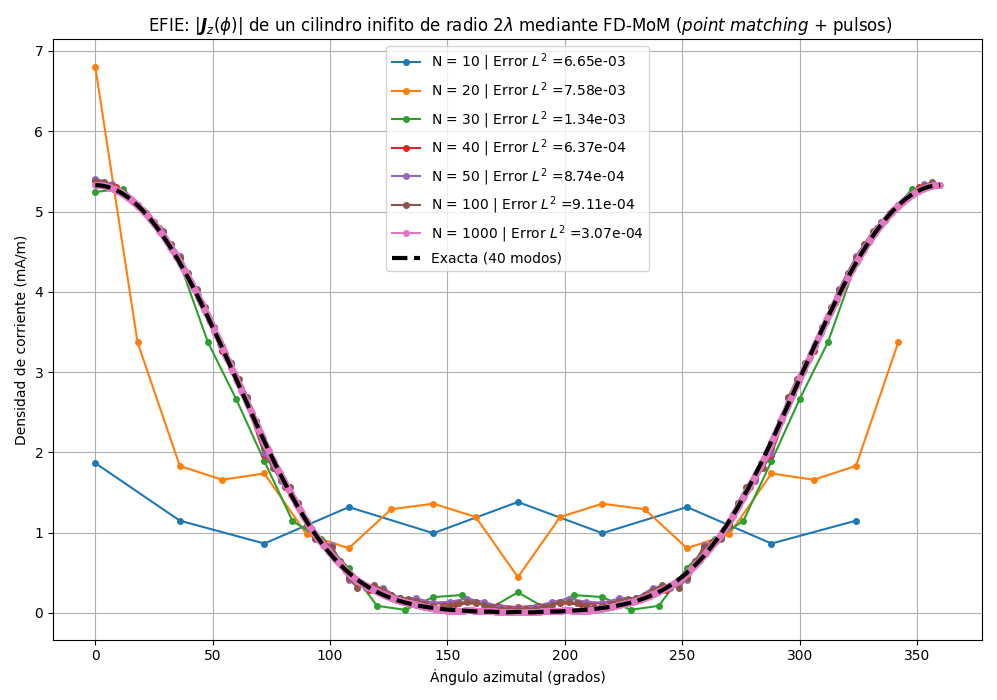
\includegraphics[width=\linewidth]{CorrientesEFIE.png}
    \caption{Módulo de la densidad de corriente superficial inducida $|J_z(\phi)|$ en función del ángulo azimutal para varios valores de $N$. El error se toma como la norma $L^2$ de la diferencia entre la solución analítica \ref{Jexacta} y la numérica descrita en la sección \ref{efienum}.}
    \label{fig:corriente}
\end{subfigure}

\vfill

\begin{subfigure}{0.95\textwidth}
    \centering
    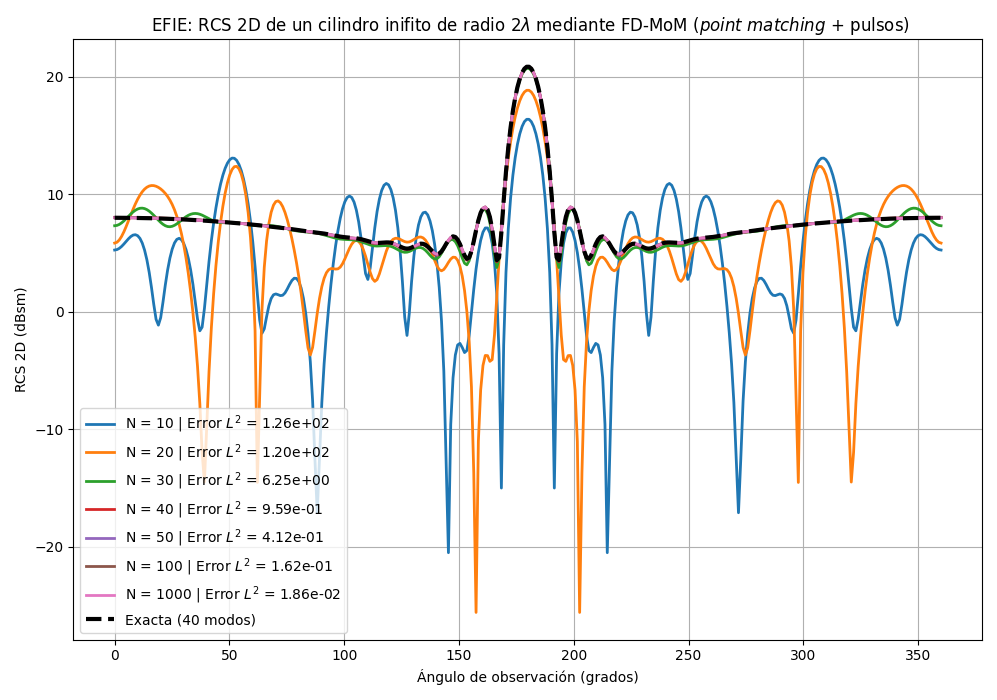
\includegraphics[width=\linewidth]{RCS2DEFIE.png}
    \caption{Sección eficaz radar bidimensional $\sigma_{2D}(\phi)$ en escala logarítmica (dBsm) en función del ángulo de observación para varios valores de $N$. El error se toma como la norma $L^2$ de la diferencia entre la solución analítica \ref{Eexacto} y la numérica descrita en la sección \ref{efienum}. Para la evaluación de $\boldsymbol{E}$ en campo lejano se usa la expresión \ref{Elejano} con $\rho = 1000 \cdot 2\lambda$.
    }
    \label{fig:rcs}
\end{subfigure}

\caption{Resultados numéricos obtenidos mediante FD-MoM para la EFIE en polarización TM para un cilindro conductor PEC con radio $a = 2\lambda$ iluminado por la onda plana incidente \ref{ondaplanaincidente} con $\phi^i=0^\circ$. La discretización en el ángulo es $2\pi a/N$. Se toman unidades normalizadas en la longitud de onda con $\lambda = 1$.}
\label{fig:resultadosEFIE}
\end{figure}










\subsection{MoM MFIE}
\label{mfienum}

En el caso de funciones base tipo pulso y \textit{point matching} solo la primera integral de \ref{ZMFIE} contribuye a los autotérminos

$$
    Z^{MFIE}_{mm} = \frac{1}{2}.
$$

La segunda integral contribuye a los términos no diagonales, usando la aproximación del centroide

$$
    Z^{MFIE}_{mm} = (\boldsymbol{\hat{n}}_m \cdot \boldsymbol{\hat{R}}_{mn}) \frac{jk\Delta l}{4} H_1^{(2)}\!\left( k \lvert \boldsymbol{\rho}_m - \boldsymbol{\rho}_n \rvert \right)
$$

Donde en el caso del cilindro $\boldsymbol{\hat{n}}_m \cdot \boldsymbol{\hat{R}}_{mn} = \frac{\rho_m}{a} \frac{\rho_m - \rho_n}{|\rho_m - \rho_n|}$ y el vector tangente es $\boldsymbol{\hat{t}} (\boldsymbol{\rho}) = sin\phi \boldsymbol{\hat{x}} - cos\phi \boldsymbol{y},$ por lo que la matriz $Z$ vuelve a ser circular.\\

Finalmente, el vector excitación es

$$
    V^{MFIE}_m = -\frac{1}{\eta} (sin\phi_m sin\phi^i + cos\phi_m cos\phi^i) e^{jk (x_m cos\phi^i + y_m sin\phi^i)}.
$$


\subsubsection{Resultados}




En la figura \ref{fig:resultadosMFIE} se muestran los resultados numéricos obtenidos mediante FD-MoM de la EFIE, junto con la solución analítica dada por \ref{Eexacto}, para la corriente inducida y la sección eficaz radar bidimensional de un cilindro infinito de radio $a = 2\lambda$. Se representan distintas discretizaciones del contorno ($\Delta \phi = 2\pi a/ N$) así como el error medido mediante la norma $L^2$.

En la distribución de corriente superficial se observa que para valores pequeños de $N$ la solución numérica presenta fuertes desviaciones a la solución exacta, especialmente en los extremos de esta. Al aumentar el número de segmentos, la corriente converge gradualmente hacia la solución analítica. A partir de $N \geq 40$ desaparecen las grandes oscilaciones, y para discretizaciones $N = 100$ y $N = 1000$ se obtiene mayor correspondencia, con errores del orden de $10^{-4}$.

Por el contrario, en el caso de la sección eficaz radar bidimensional se aprecia una convergencia más lenta y menos regular. Para discretizaciones gruesas aparecen oscilaciones espurias de gran amplitud y desviaciones significativas en los mínimos y máximos. Aunque dichas oscilaciones se reducen al aumentar $N$, incluso para $N = 1000$ persisten pequeñas diferencias respecto a la solución exacta, con un error del orden de $10^{-1}$.

Esto puede explicarse a través naturaleza de la formulación MFIE, que involucra derivadas de la función de Green, lo que la dota de un comportamiento menos regular. El uso de funciones base tipo pulso y el \textit{point matching} no proporciona una representación suficientemente suave de la solución. El uso de por ejemplo funciones triangulares que si tienen una divergencia bien definida mejoraría el resultado al capturar los cambios en la función de Green.












\newpage
\begin{figure}[H]
\centering

\begin{subfigure}{0.95\textwidth}
    \centering
    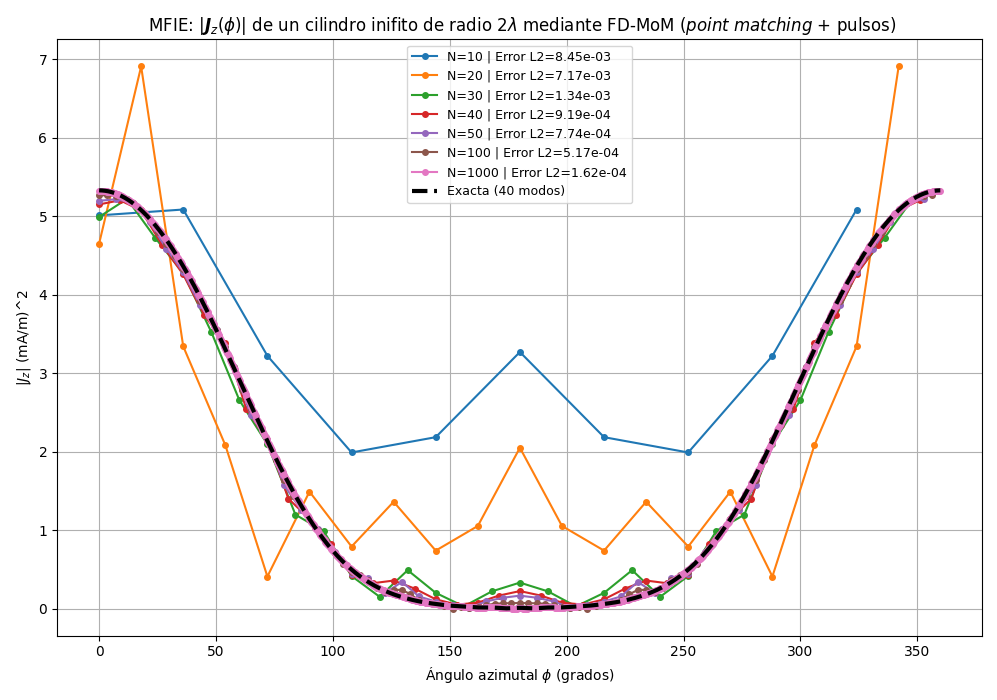
\includegraphics[width=\linewidth]{CorrientesMFIE.png}
    \caption{Módulo de la densidad de corriente superficial inducida $|J_z(\phi)|$ en función del ángulo azimutal para varios valores de $N$. El error se toma como la norma $L^2$ de la diferencia entre la solución analítica \ref{Jexacta} y la numérica descrita en la sección \ref{mfienum}.}
    \label{fig:corriente}
\end{subfigure}

\vfill

\begin{subfigure}{0.95\textwidth}
    \centering
    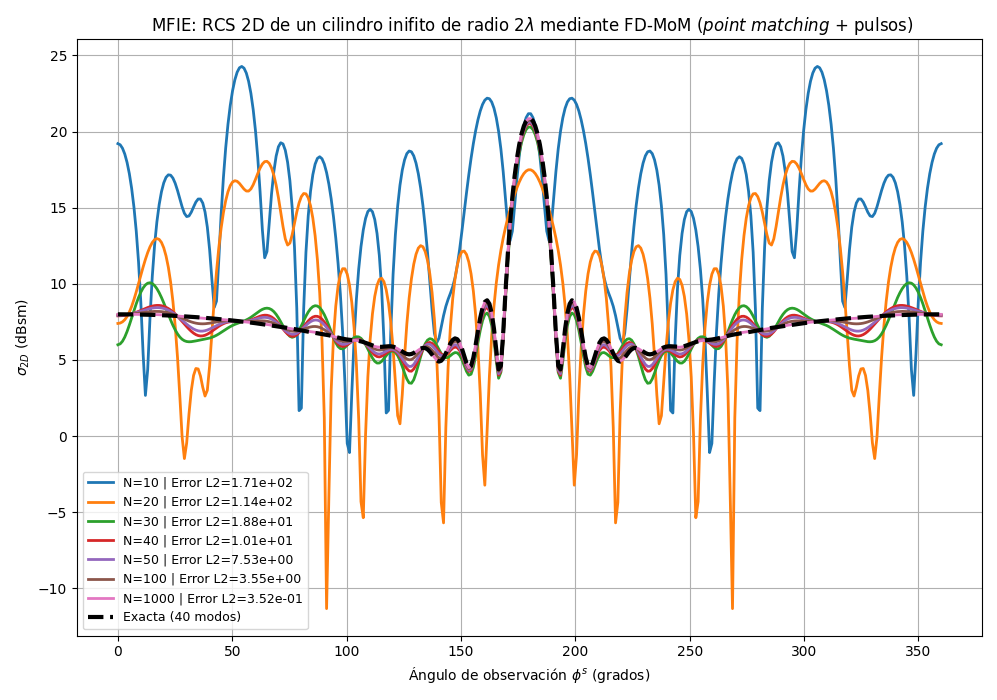
\includegraphics[width=\linewidth]{RCS2DMFIE.png}
    \caption{Sección eficaz radar bidimensional $\sigma_{2D}(\phi)$ en escala logarítmica (dBsm) en función del ángulo de observación para varios valores de $N$. El error se toma como la norma $L^2$ de la diferencia entre la solución analítica \ref{Eexacto} y la numérica descrita en la sección \ref{mfienum}. Una vez obtenidas las corrientes mediante la MFIE se obtiene el campo $E$ en régimen lejano con \ref{Elejano} y $\rho = 1000 \cdot 2\lambda$.
    }
    \label{fig:rcs}
\end{subfigure}

\caption{Resultados numéricos obtenidos mediante FD-MoM para la MFIE en polarización TM para un cilindro conductor PEC con radio $a = 2\lambda$ iluminado por la onda plana incidente \ref{ondaplanaH} con $\phi^i=0^\circ$. La discretización en el ángulo es $2\pi a/N$. Se toman unidades normalizadas en la longitud de onda con $\lambda = 1$.
}
\label{fig:resultadosMFIE}
\end{figure}





\newpage






\section{Conclusión}

En este trabajo se ha abordado la resolución numérica de un problema de dispersión electromagnética bidimensional mediante el Método de los Momentos, aplicándolo a las formulaciones EFIE y MFIE para un cilindro conductor perfecto en polarización TM.

Los resultados obtenidos muestran que la formulación EFIE presenta un comportamiento numéricamente estable y una convergencia rápida hacia la solución analítica al aumentar el número de segmentos $N$. A partir de discretizaciones elevadas la corriente superficial inducida y la sección eficaz radar bidimensional reproducen con elevada precisión la solución exacta, alcanzándose errores del orden de $10^{-4}$ cuando se emplean funciones base tipo pulso y \textit{point matching}.

En el caso de la formulación MFIE, se observa una buena convergencia en la corriente superficial, similar a la obtenida mediante EFIE. Sin embargo, la convergencia de la RCS resulta más lenta y presenta una mayor sensibilidad a la discretización. Incluso para valores elevados de $N$, persisten pequeñas discrepancias respecto a la solución analítica, reflejadas en errores superiores a los obtenidos con EFIE.

Este comportamiento se debe a la naturaleza de la MFIE, que involucra derivadas del núcleo integral y, por tanto, amplifica los errores asociados a discretizaciones poco suaves. El uso de funciones pulso y \textit{point matching} limita la precisión en la formulación.

Los resultados indican que la EFIE proporciona una mayor precisión global, mientras que la MFIE requiere esquemas de discretización más complejos para alcanzar un nivel de exactitud comparable. Por tanto, para aplicaciones prácticas con discretizaciones sencillas, la EFIE constituye una opción más adecuada en el análisis de dispersión electromagnética bidimensional.



















\newpage

\bibliographystyle{plain}
\bibliography{bibliografia}





\end{document}